\chapter{App}
\section{Registrierung}
Bei der Registrierung gibt der Benutzer seinen gewünschten Benutzernamen und sein Passwort ein. Der Benutzername und der SHA1-Hash des Passworts wird dann an den Server gesendet und sofern der Benutzername nicht bereits existiert wird der neue Benutzer angemeldet. Dies wird dem Benutzer mit einer Nachricht mitgeteilt. Der Benutzer kann sich nun anmelden.

\begin{capfigure}[App - Registrierung]
	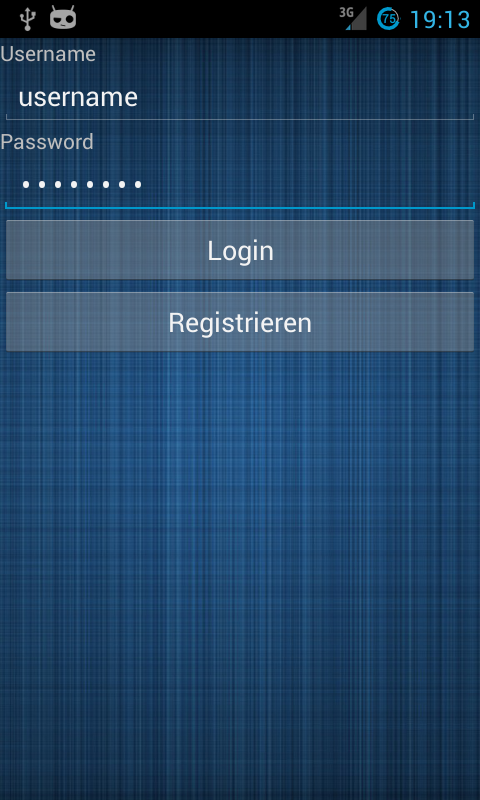
\includegraphics[width=6cm]{images/app/login}
\end{capfigure}


\section{Anmeldung}
Ein bereits registrierter Benutzer kann sich analog zur Registrierung anmelden. War die Anmeldung erfolgreich bekommt die App ein Token und wechselt in das Hauptmenü.

\section{Hauptmenü}
Über das Hauptmenü lassen sich die verschiedenen Funktionen der App Aufrufen. Dazu gehört der Chat, die Anzeige der \glspl[{poi}, Navigation und der Spiele.

\begin{capfigure}[App - Hauptmenü]
	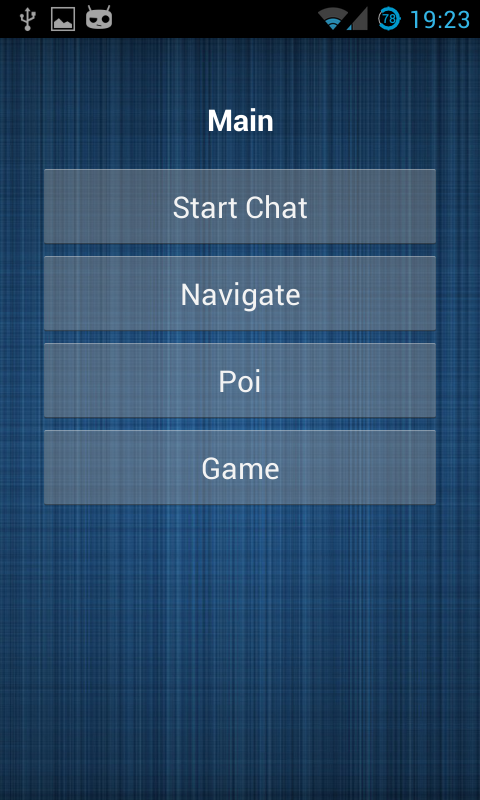
\includegraphics[width=6cm]{images/app/main_menu}
\end{capfigure}

\section{Chatsystem}
Um den Nutzern der App die Möglichkeit zu bieten miteinander zu kommunizieren wurde ein Nachrichtensystem implementiert. Dieses ermöglicht es den Nutzern der App über diese miteinander zu kommunizieren und ermöglicht es Freunde zur Freundesliste hinzuzufügen.\\
Die Kommunikation erfolgt über den zentralen Server. Alle gesendeten Nachrichten eines Nutzers werden dort gespeichert und können von den Kommunikationspartnern abgerufen werden. \\
Neben den Nachrichten wird auch die Freundesliste auf dem Server abgelegt.

\subsection{Freundesliste}
Startet man den Chat über das Hauptmenü, so erhält man zunächst die Möglichkeit neue Freunde (andere regstrierte Benutzer) durch Eingabe deren Namen zur Freundesliste hinzuzufügen. In der selben Ansicht wird die Freundesliste angezeigt. Sobald die Freundesliste geöffnet wird oder ein neuer Freund hinzugefügt wurde, wird die Liste vom Server abgerufen und angezeigt.
\begin{capfigure}[App - Freundesliste]
	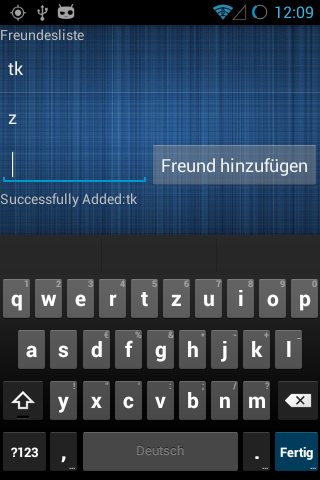
\includegraphics[width=6cm]{images/app/friendlist}
\end{capfigure}
Durch Tippen auf einen Freund in der Freundesliste öffnet man die Kommunikationsansicht, den eigentlichen Chat.


\subsection{Chat}
Wurde der Chat mit jemandem aus der Freundesliste geöffnet, werden bereits versendete und empfangene Nachrichten vom Server abgerufen und angezeigt.\\
In das Eingabefeld lassen sich dann Nachrichten eingeben und durch antippen von \textit{Nachricht senden} übertragen. Je nachdem ob man Empfänger oder Sender einer jeweiligen Nachricht ist, wird die Nachricht farbig dargestellt.
\begin{capfigure}[App - Chat]
	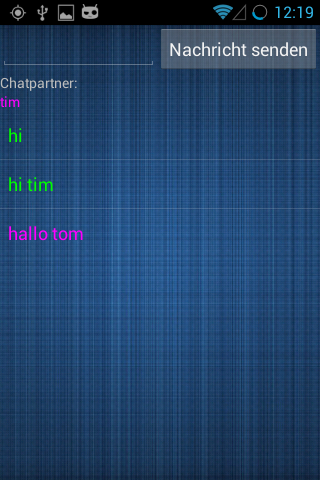
\includegraphics[width=6cm]{images/app/chat}
\end{capfigure}
Dank dieser Funktionalität wird es den Nutzern der App ermöglicht auf einfache Art und Weise Kontaktpflege zu betreiben und sich beispielsweise für ein Treffen bei einem der \glspl{poi} zu verabreden.\\
Aufgrund der integrierten Nachrichtenlösung ist es möglich, dass sich die Nutzer untereinander verständigen können, ohne persönlichen Daten veröffentlichen zu müssen.

\section{Kompass}
Neben dem Kompass werden in der KompassView noch weitere Daten dargestellt. Es wird die aktuelle GPS-Position in Form von Longitude und Latitude angezeigt.

\begin{capfigure}[App - Kompass]
	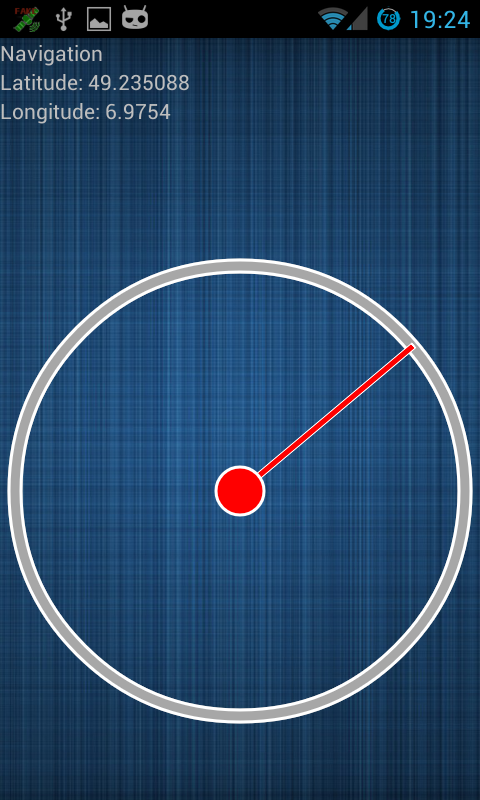
\includegraphics[width=6cm]{images/app/compass}
\end{capfigure}

\section{Navigation}
Für die Navigation wird die KompassView verwendet. Wenn sich die KompassView im Navigationsmodus befindet wird zusätzlich die Richtung zum Ziel als auch die Entfernung angezeigt.

\begin{capfigure}[App - Navigation]
	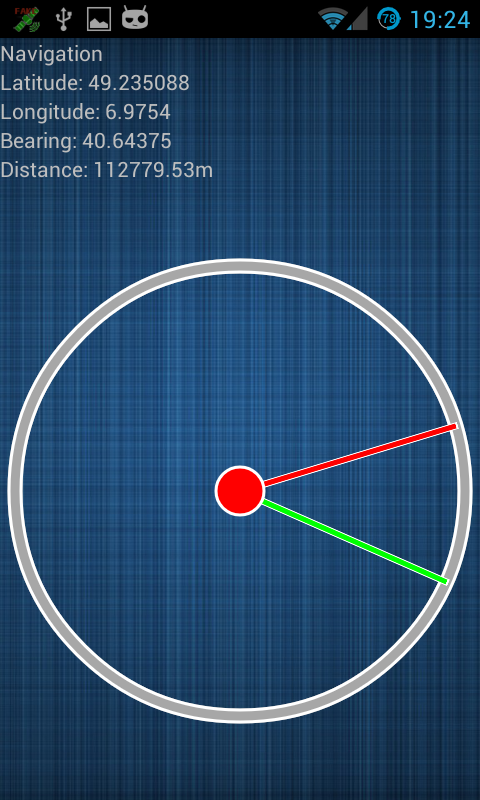
\includegraphics[width=6cm]{images/app/navigation}
\end{capfigure}

Für die Navigation wird auf Funktionen des Android-Frameworks zurückgegriffen. Über diese Funktionen wird die Distanz berechnet und das Bearing. Bearing gibt den Winkel zum Nordpol an.

\section{Points of Interest}
Die App verbindet \glspl{poi} mit bestimmten Ereignissen wie einem Spiel. Ein \gls{poi} besteht im Wesentlichen aus Koordinaten, Namen und Eigenschaft.  Die \glspl{poi} werden ebenfalls in der Datenbank gespeichert und können über den Punkt \textit{\gls{poi}} aus dem Hauptmenü aufgerufen werden. Wählt man einen \gls{poi} aus der Liste durch antippen aus, werden einem die Details angezeigt wie in folgender Abbildung zu sehen ist.
\begin{capfigure}[App - POI detailliert]
	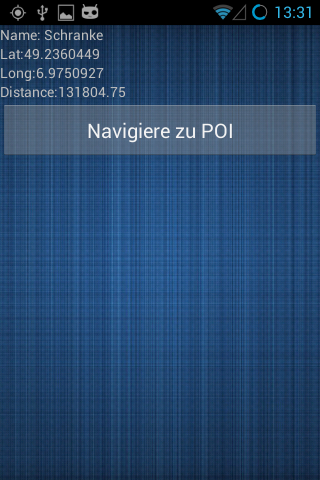
\includegraphics[width=6cm]{images/app/poidetail}
\end{capfigure}
Dazu gehören neben Längengrad, Breitengrad und Namen des \gls{poi} auch die Distanz zum POI in Metern. Mit dem Button \textit{Navigiere zu POI} wird die Navigation welche zuvor beschrieben wurde aufgerufen.

\section{Spiele}
Ruft man im Hauptmenü den Punkt \textit{Game} auf, so werden die vorhandenen Spiele dargestellt, aktuell gibt es jedoch nur \gls{rpssl}. Die Auswahl selber wurde als einfaches Buttonmenü implementiert und beinhaltet nur ein Element.
\begin{capfigure}[App - Spielauswahl]
	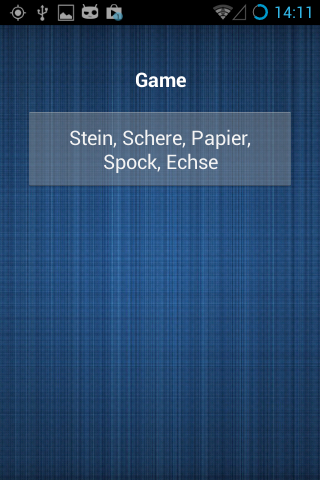
\includegraphics[width=6cm]{images/app/gamelist}
\end{capfigure}


\subsection{Rock, Paper, Scissors, Lizzard, Spock}

\begin{capfigure}[App - Rock, Paper, Scissors, Lizzard, Spock]
	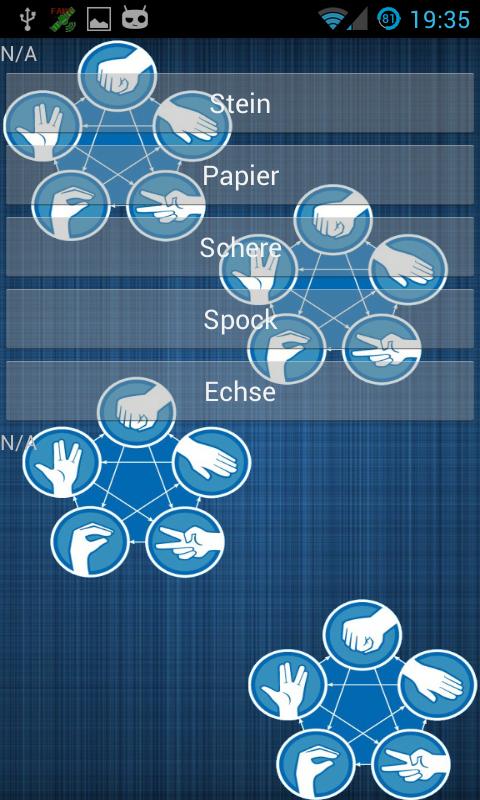
\includegraphics[width=6cm]{images/app/rpssl}
\end{capfigure}



\subsubsection{Spielablauf}
\TODO{Im Details beschreiben wie ein Spiel erzeugt wird und gespielt wird}

